
\section{Resultados}

\subsection{Red de interacciones inicial}


\begin{figure}[h] % [h] indica que queremos la imagen aquí, en la posición actual
	\centering
	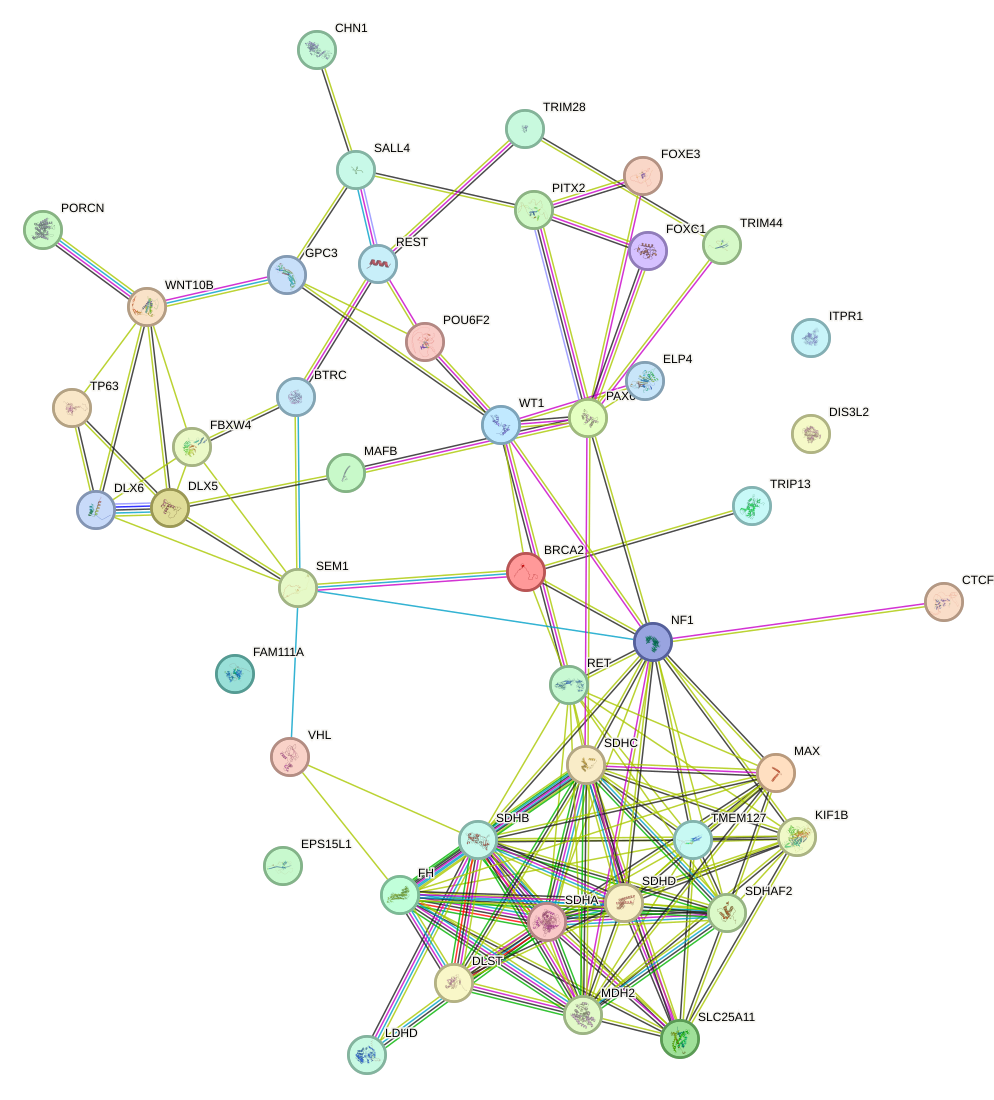
\includegraphics[width=1\textwidth]{figures/red_interaccion_aniridia.png} % Especifica la ruta y el tamaño
	\caption{Red de interacción con los genes asociados al fenotipo HP:0000526} % Agrega una leyenda si deseas
	\label{fig:mi-imagen} % Etiqueta para referenciar la imagen en el texto
\end{figure}

\subsection{Propagación de la red}

A partir de los genes semilla WNT10B, WT1, SEM1, PAX6, y NF1, se generó una red de interacciones proteína-proteína (PPI) utilizando datos de STRINGdb. Se estableció un umbral de puntaje de interacción de 700 para incluir únicamente conexiones de alta confianza. La red inicial centrada en los genes semilla fue posteriormente expandida mediante el algoritmo DIAMOnD, incluyendo 200 nodos adicionales que se encuentran altamente conectados con los genes semilla y entre sí.

La red generada señala importantes interacciones entre los genes semilla y otros desconocidos (como la relación WNT10B - TGFB2), lo cual permite continuar el estudio hacia el objetivo del artículo.

\subsection{Clustering}

\begin{figure}[h] % [h] indica que queremos la imagen aquí, en la posición actual
	\centering
	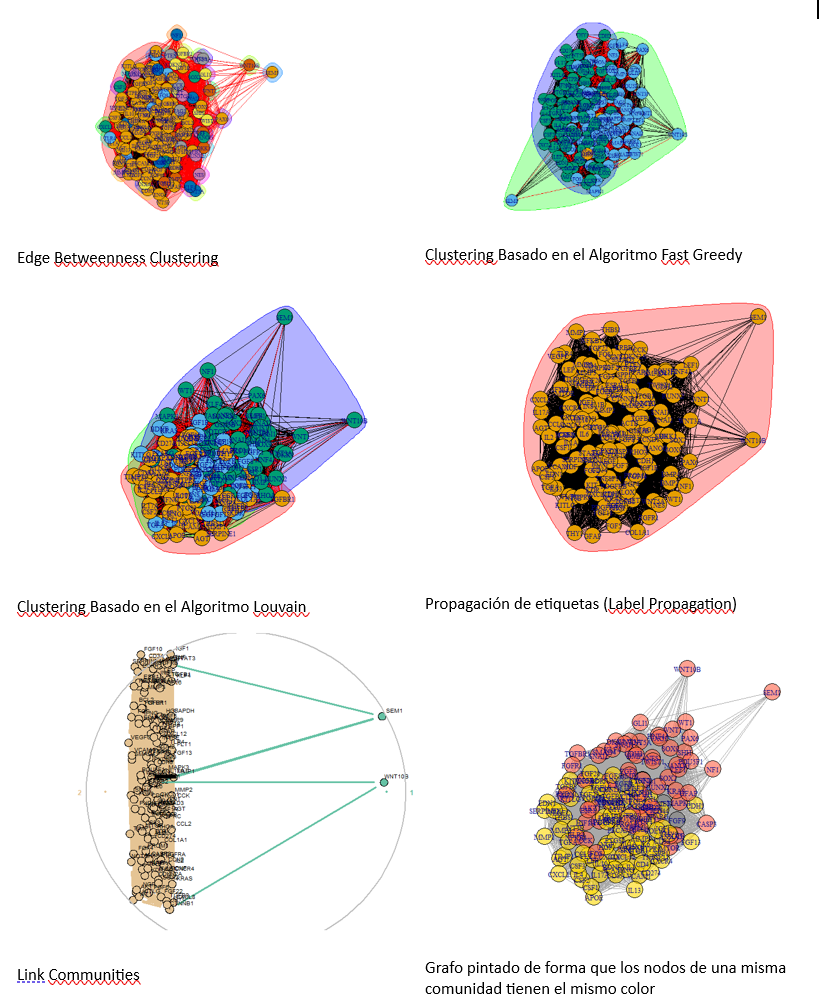
\includegraphics[width=1\textwidth]{figures/toda_figuras_clustering.png}
	\caption{Figuras obtenidas al aplicar clustering con distintos métodos}
	\label{clustering}
\end{figure}

Principalmente el estudio de los resultados se centrará en los genes semilla (WNT10B, WT1, SEM1, PAX6, NF1). En común, se puede observar que SEM1 aparece en varisa posiciones destacadas en los grafos; WT1 y PAX6 están en regiones densas (centrales) de las comunidades, lo que infica que tienen muchas conexiones internas; y NF1 se sitúa en los bordes de las comunidades, por lo que podría actuar como puente entre diferentes comunidades; y WNT10B también es central en algunas comunidades.